\documentclass[12pt,oneside,a4paper]{report}
\usepackage[OT4]{polski}
\usepackage[cp1250]{inputenc}
\usepackage{geometry}
\usepackage{latexsym}
\usepackage{graphicx}
\usepackage{float}
\usepackage{indentfirst}
\usepackage{hyperref} % paczka do hiper��czy
\usepackage{geometry}
%\usepackage{showframe}
\usepackage{sidecap} % paczka do wstawiania opis�w zdj��
\usepackage{wrapfig} % paczka do op�ywania zdj��
\usepackage{pdfpages}
\usepackage{listings}
\usepackage{mathrsfs}
%\usepackage{verbatim}
\lstset{language=Matlab}



\geometry{marginparwidth=0mm,
left=25mm,
right=25mm,
top=25mm,
bottom=30mm,
footskip=15mm}

%Create by Marek Ogonowski

\makeatletter %w��cza u�ycie "zmiennych" typu \author,\title

%definicja wlasnego przesuniecia PW itd.
\newcommand{\odstep}{\hspace{1,5cm}}

%zdefiniowanie komendy rysujacej linie
\newcommand{\linia}{\rule{\linewidth}{0.4mm}}

%definicja zmienej \place
\newcommand{\place}[1]{\gdef\@place{#1}}%
\newcommand{\@place}{\@latex@warning@no@line{No \noexpand\place given}}

%definicja zmiennej promotor
\newcommand{\promotor}[1]{\gdef\@promotor{#1}}%
\newcommand{\@promotor}{\@latex@warning@no@line{No \noexpand\promotor given}}

%definicja zmiennej nr albumu
\newcommand{\album}[1]{\gdef\@album{#1}}%
\newcommand{\@album}{\@latex@warning@no@line{No \noexpand\album given}}

%definicja zmiennej kierunek studi�w
\newcommand{\kierunek}[1]{\gdef\@kierunek{#1}}%
\newcommand{\@kierunek}{\@latex@warning@no@line{No \noexpand\kierunek given}}

%definicja zmiennej nr albumu
\newcommand{\specjalnosc}[1]{\gdef\@specjalnosc{#1}}%
\newcommand{\@specjalnowsc}{\@latex@warning@no@line{No \noexpand\specjalnosc given}}

%zmiana definicji strony tytu�owej
\renewcommand{\maketitle}{\begin{titlepage}

	\begin{figure}
	\vspace*{-1cm}
		\centering
		
\includegraphics[width=16 cm]{KNR.png}
		\label{fig:KNR} 
	\end{figure}
	
	\vspace*{-1,2cm}	
	\noindent\linia

	\vspace{2cm}
    
    \begin{center}
    	\LARGE {OPIS PROJEKTU}
    \end{center}
    
    \vspace{0.5cm}
    
    \begin{center}
      \Large \textsc{\@author}
    \end{center}
    
    \vspace{0.5cm}

	\begin{center}
		\LARGE \textsc{\@title}
	\end{center}

	\vspace{1,5cm}

%    \begin{flushright}
%    	\begin{minipage}{6cm}
%    		\textit{\footnotesize numer albumu:}
%    		\footnotesize {\@album} \\
%    		\textit{\footnotesize kierunek:}
%    		\footnotesize {\@kierunek} \\
%    		\textit{\footnotesize specjalno��:}
%    		\footnotesize {\@specjalnosc} \\
%    	\end{minipage}
%     \end{flushright}
     
    \vspace*{\stretch{18}}
     


    \begin{center}
	   \@place, \@date
    \end{center}

  \end{titlepage}
}
\makeatother %wy��cza u�ycie "zmiennych" typu \author,\title

\author{in�. Daniel Wlaz�o \\ in�. Marek Ogonowski}
\album{244123}
\kierunek{Automatyka i Robotyka}
\specjalnosc{Robotyka}
\title{Minotaur - Robot klasy Micromouse}
\place{Warszawa}

\begin{document}
	\maketitle
	

\linespread{1.3} 	
\tableofcontents 
	
\linespread{1.3} 	
\chapter{Zadanie}

\section{Tre�� projektu}

\begin{figure}[H]
\centering
\includegraphics[width=16 cm]{foto/SCHEMAT.png}
\caption{Schemat uk�adu regulacji}
\label{fig:ZADANIE}
\end{figure} 

Dla uk�adu regulacji o powy�szej strukturze wybra� czas pr�bkowania  \( T_p \)   oraz dobra� tak transmitancj� regulatora dyskretnego \( R(z) \) , aby otrzyma� uk�ad regulacji spe�niaj�cy nast�puj�ce wymagania:

\begin{itemize}
\item uchyby po�o�eniowy i pr�dko�ciowy w stanie ustalonym s� najmniejsze z mo�liwych do osi�gni�cia,
\item  wymuszenia \( r \) o maksymalnej pr�dko�ci \( r_1 \)  i maksymalnym przyspieszeniu \( r_2 \) s� przenoszone
z uchybem nie wi�kszym ni� \( \varepsilon \) ,
\item  odpowied� uk�adu regulacji na skok jednostkowy charakteryzuje si� ma�� oscylacyjno�ci� i niezbyt
du�ym czasem ustalania, co jest zwi�zane z przyj�t� przez projektanta maksymaln� wielko�ci�
piku rezonansowego \( M_p \) uk�adu zamkni�tego,
\item  modu� sterowania \( u \) nie przekracza rozs�dnej granicy.
\end{itemize}

Projekt powinien przedstawia� co najmniej:
\begin{itemize}
\item transmitancj� i r�wnanie r�nicowe wybranego regulatora,
\item charakterystyki cz�stotliwo�ciowe transmitancji: \\
\begin{center}
\( G(j\omega), HG^*(j\omega), HG^*(jv),\) \\
\( L^*(jv) = R^*(jv)HG^*(jv), \)
\end{center}
\item charakterystyk� Nyquista zaprojektowanego uk�adu otwartego,
\item przyj�t� przez projektanta maksymaln� wielko�ci� piku rezonansowego \( M_p \) uk�adu zamkni�tego,
\item charakterystyk� amplitudow� funkcji wra�liwo�ci \( |S*(j\omega)| \) oraz charakterystyk� amplitudow� dope�niaj�cej funkcji wra�liwo�ci (transmitancji uk�adu zamkni�tego) \( |T*(j\omega)| \), charakterystyk�
amplitudow� funkcji wra�liwo�ci sterowania \( |R*(j\omega)| \) , zaprojektowanego systemu pokazuj�ce,
�e spe�niono postawione wymagania w dziedzinie cz�stotliwo�ciowej,
\item odpowiedzi uk�adu regulacji na:
\begin{itemize}
\item skok jednostkowy,
\item skok jednostkowy o amplitudzie \( (r_1)^2/r_2 \) ,
\item wymuszenie harmoniczne: \\
\begin{center}
\( t \mapsto r(t) = \frac{(r_1)^2}{r_2} sin(\frac{r_2}{r_1}t)  \) \\
\end{center}
\item wymuszenie o trapezoidalnym przebiegu pr�dko�ci i pr�dko�ci maksymalnej r�wnej \( r_1 \)
oraz przyspieszeniu maksymalnym r�wnym \( r_2 \) ,
\item sterowanie wywo�ane powy�szym wymuszeniem, pokazuj�ce, �e spe�niono wymagania w dziedzinie czasowej.
\end{itemize}
\end{itemize}
\section{Dane do projektu}
Zestaw numer 16:
\begin{itemize}
\item Transmitancja:
\begin{center}
\( G(s)= \frac{150}{s(1.12s+1)(0.224s+1)}  \) \\
\end{center}
\item Maksymalna pr�dko��:
\begin{center}
\( r_1=1 \) \\
\end{center}
\item Maksymalne przyspieszenie:
\begin{center}
\( r_2=0.8 \) \\
\end{center}
\item Dok�adno��
\begin{center}
\( \varepsilon=0.005 \) \\
\end{center}
\end{itemize}	 

\chapter{Wst�p}

Rozdzia� ten powsta� we wsp�pracy z kol. Jakubem Pierewojem, ze wzgl�du na komplementarno�� obu prac - obie traktuj� o budowie robot�w w kategorii Ketchup House - niniejsza zawiera opis konstrukcji mechanicznej i elektronicznej natomiast praca kol. Jakuba \cite{inzynierkaKuby} jego sterowanie i programowanie.

\section{Robotyka mobilna}

Robotyka mobilna to do�� szczeg�lny dzia� robotyki, o niewyra�nych granicach. Istnieje wiele definicji robot�w mobilnych Wg E. Jezierskiego \cite{test1}, robot mobilny to kompozycja r�norodnych fizycznych i informatycznych sk�adnik�w tworz�ca 4 podstawowe podsystemy: \\
\begin{itemize}
	\item Ruchu (locomotion),
	\item Detekcji (sensing),
	\item Wnioskowania (reasoning),
	\item Komunikacji (communication).
\end{itemize}

Natomiast wg Maji Mataric \cite{mataric}, jest to autonomiczny system, kt�ry istnieje w �wiecie fizycznym, nie jest zamocowany w jednej, ustalonej lokalizacji oraz ma mo�liwo�� detekcji otoczenia i dzia�ania na nim, aby osi�gn�� pewne cele.

\begin{figure}[H]
\centering
\includegraphics[width=11 cm]{zdjecia/SEEKUR.jpg}
\caption{Robot SEEKUR � przyk�ad robota mobilnego}
\label{fig:SEEKUR}
\end{figure} 

Niezale�nie od przyj�tej definicji, robotyka mobilna jest bardzo szerokim i niejednorodnym dzia�em. Roboty mobilne, w zale�no�ci od �rodowiska w jakim dzia�aj� mo�na podzieli� na kilka kategorii. Wyr�niamy roboty lataj�ce, p�ywaj�ce, oraz poruszaj�ce si� na l�dzie. 

Roboty l�dowe mo�na podzieli� ze wzgl�du na spos�b przemieszczania. Istniej� mobilne roboty krocz�ce oraz ko�owe (w tym poruszaj�ce si� na g�sienicach). Ka�de z rozwi�za� posiada zar�wno wady jak i zalety. Roboty ko�owe mog� rozwija� wi�ksze pr�dko�ci w por�wnaniu z robotami krocz�cymi. Z kolei roboty krocz�ce lepiej funkcjonuj� na nier�wnym pod�o�u.

\section{Robotyka amatorska}

Robotyka amatorska jest do�� szczeg�lnym dzia�em robotyki. Jest to dziedzina zajmuj�ca si� robotami mobilnymi, kt�re maj� za zadanie konkurowa� ze sob� podczas zawod�w w jednej z kilku dyscyplin. Do najbardziej znanych i popularnych konkurencji mo�na zaliczy� m.in.:
\begin{itemize}
	\item Zawody Line Follower � w kt�rych roboty maj� za zadanie porusza� si� jak najszybciej po torze. Tor wyznaczany jest przez ciemn� lini� umieszczon� na jasnej planszy. Roboty s� startowane pojedynczo, zwyci�a robot, kt�ry bezb��dnie przejedzie tras� w najkr�tszym czasie. W mniej �kanonicznej� odmianie tego typu zawod�w na trasie umieszczane s� przeszkody (np. podjazdy, kurtyny, �ciany), kt�re maj� utrudni� robotom przejazd.
	\begin{figure}[H]
	\centering
	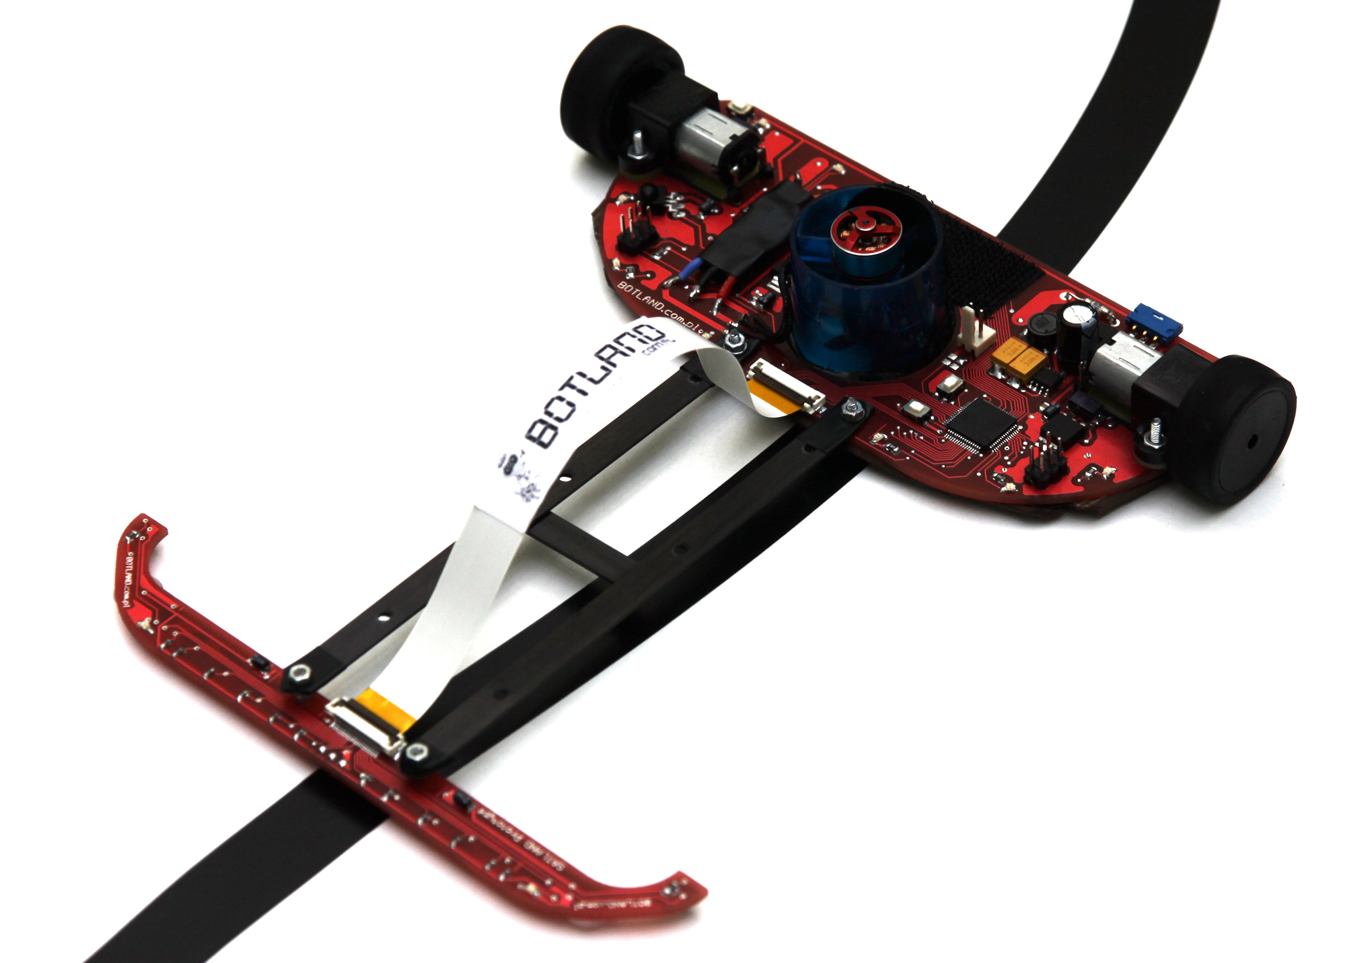
\includegraphics[width=10 cm]{zdjecia/IMPACT.png}
	\caption{Impact � przyk�ad Line Followera \cite{LF}}
	\label{fig:IMPACT}
	\end{figure} 
	\item Zawody MicroMouse - w kt�rych robot, czyli "mysz" ma za zadanie w jak najkr�tszym czasie rozwi�za� labirynt. Klasyczny labirynt z�o�ony jest z 256 (16x16) kwadratowych element�w o wymiarach 180x180 mm pooddzielanych mi�dzy sob� �ciankami. Rozwi�zanie labiryntu polega na jego przeszukaniu i odnalezieniu najkr�tszej �cie�ki z kwadratu startowego (jest to jeden z naro�nik�w labiryntu) do �rodka labiryntu. Wygrywa ta "mysz", kt�ra zrealizuje zadanie w najkr�tszym czasie. 
	\begin{figure}[H]
	\centering
	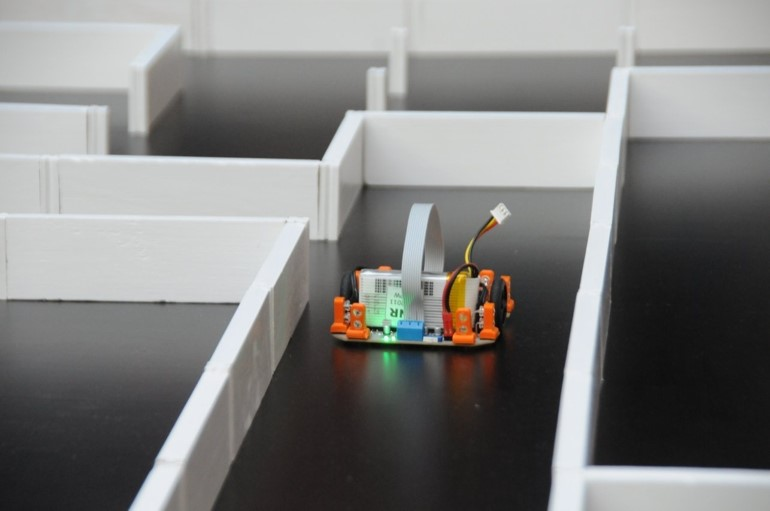
\includegraphics[width=10 cm]{zdjecia/TEZEUSZ.jpg}
	\caption{Tezeusz � przyk�ad MicroMouse�a}
	\label{fig:TEZEUSZ}
	\end{figure} 
	\item Zawody Sumo (oraz ich pochodne � MiniSumo, MicroSumo...) � w kt�rych roboty umieszczane na arenie zwanej dohyo (dod�o), ich celem jest zlokalizowanie, zaatakowanie i zepchni�cie z maty przeciwnika. Roboty nie mog� zawiera� urz�dze� zak��caj�cych uk�adu sterowania przeciwnika, b�yskaj�cych �wiate� ani urz�dze� blokuj�cych ruch. W zale�no�ci od konkurencji limitowane s� waga i wymiary konstrukcji (np. w MiniSumo waga nie mo�e przekracza� 0,5 kg).
	\begin{figure}[H]
	\centering
	\includegraphics[width=10 cm]{zdjecia/MM.png}
	\caption{M\&M's � przyk�ady robot�w MicroSumo}
	\label{fig:MnM}
	\end{figure} 
	\item Zawody PuckCollect � w kt�rej roboty s� umieszczane na planszy, na kt�rej porozrzucano niewielkie, kolorowe kr��ki (z ang. puck). Na pocz�tku ka�dego pojedynku, ka�demu robotowi zostaje przydzielony kolor � czerwony lub niebieski, po czym roboty s� umieszczane w bazach o odpowiadaj�cym im kolorze. Celem jest dostarczenie do bazy jak najwi�cej puck�w wybranego koloru.
	\begin{figure}[H]
	\centering
	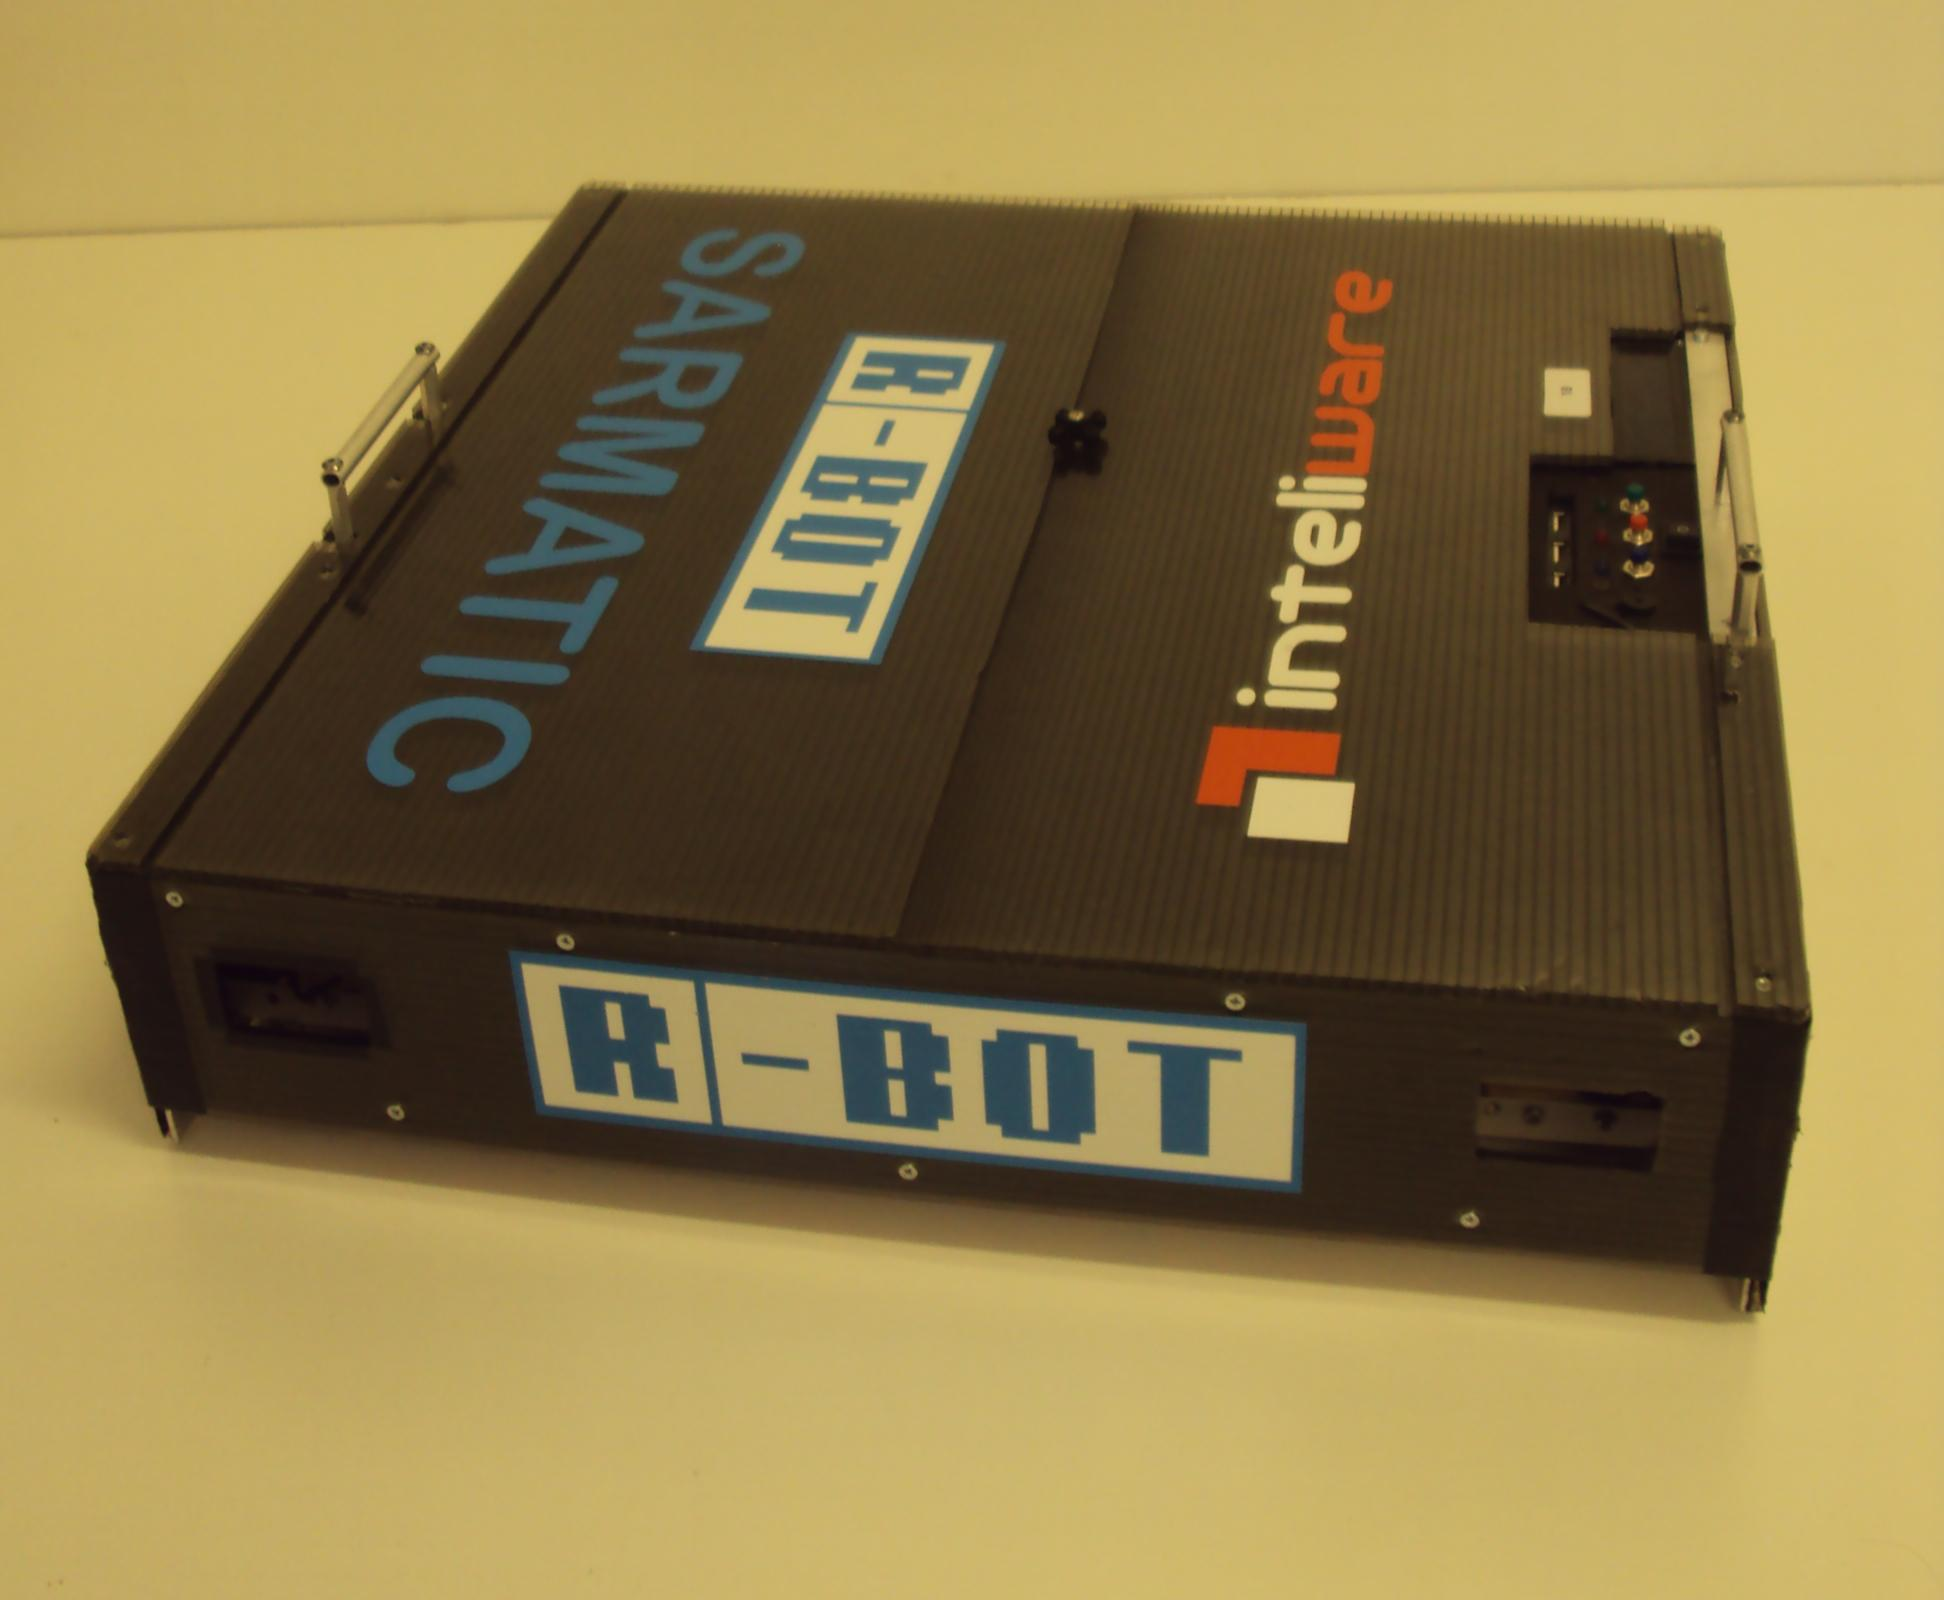
\includegraphics[width=10 cm]{zdjecia/SARMATIC.png}
	\caption{Sarmatic � przyk�ad robota kategorii PuckCollect \cite{PUCK}}
	\label{fig:SARMATIC}
	\end{figure} 
\end{itemize}

\section{Zawody Ketchup House}
\subsection{Historia dyscypliny}

Ketchup House (znana tak�e jako Tomato House i V sklade ke�upu) jest stosunkowo m�od�, lecz pr�nie rozwijaj�c� si� konkurencj� zmaga� autonomicznych robot�w mobilnych. Pierwsze zawody rozegrano w Stanach Zjednoczonych na pocz�tku XXI wieku. Stamt�d przyw�drowa�a do Czech i S�owacji, gdzie cieszy si� zdecydowanie najwi�ksz� popularno�ci�. 
	\begin{figure}[H]
	\centering
	\includegraphics[width=10 cm]{zdjecia/ISTROBOT.png}
	\caption{Zawody ISTROBOT w Bratys�awie \cite{ISTRO}}
	\label{fig:ISTRO}
	\end{figure} 
	
	Najwi�ksze i ciesz�ce si� ogromnym zainteresowaniem publiczno�ci zawody to Istrobot (organizowany przez Politechnik� S�owack� w Bratys�awie) oraz Robotic Day (organizowane przez Uniwersytet Karola w Pradze).
	
	\begin{figure}[H]
	\centering
	\includegraphics[width=10 cm]{zdjecia/ROBOTICDAY.jpg}
	\caption{Zawody Robotic Day w Pradze \cite{ROBOTIC}}
	\label{fig:ISTRO}
	\end{figure} 
	
	
\subsection{Zasady rozgrywki}

Ketchup House jest zdecydowanie najbardziej nieprzewidywaln� i widowiskow� konkurencj� odbywaj�c� si� na zawodach konstruktorskich. ��czy w sobie cechy 4 pozosta�ych kategorii rozgrywanych na tego typu imprezach (Line follower, Micro mouse, Sumo, Puck Collect).

W ka�dej, trwaj�cej 3 minuty rozgrywce udzia� bior� 2 roboty. Polem ich zmaga� jest bia�a, kwadratowa plansza o wymiarach min. 1,8x1,8m. Na planszy znajduje si�  10 czarnych linii (5 poziomych i 5 pionowych) o szeroko�ci 12mm, tworz�c kwadrat o wymiarach 1,2x1,2m, podzielony na 16 mniejszych kwadrat�w o wymiarach 0,3x0,3m. 
	\begin{figure}[H]
	\centering
	\fbox{ \includegraphics[width=9 cm]{zdjecia/PLANSZA.png} }
	\caption{Plansza, na kt�rej odbywaj� si� zawody (wymiary w mm)}
	\label{fig:PLANSZA}
	\end{figure} 

Na skrzy�owaniach umieszczane s� puszki z tytu�owym keczupem. S� to typowe stalowe puszki o �rednicy 53 mm, wysoko�ci 74 mm i masie ok. 163 g.
	\begin{figure}[H]
	\centering
	\includegraphics[width=5 cm]{zdjecia/PUSZKA.jpg}
	\caption{Przyk�adowa puszka u�ywana podczas zawod�w}
	\label{fig:PUSZKA}
	\end{figure} 

W ka�dej, trwaj�cej 3 minuty potyczce bior� udzia� 2 roboty. Ich zadaniem jest przemieszczenie puszek na swoj� lini� �domow��.
 
Na pocz�tku rozgrywki na planszy znajduje si� 5 puszek. 2 z nich, zaznaczone na rys. 10 na zielono, znajduj� si� w ustalonych pozycjach (skrzy�owania C2 oraz C4). Po�o�enie 3 pozosta�ych puszek jest losowane tu� przed rozpocz�ciem pojedynku. 
	\begin{figure}[H]
	\centering
	\fbox{ \includegraphics[width=8 cm]{zdjecia/PLANSZA2.png} }
	\caption{Plansza startowa z zaznaczonymi robotami oraz miejscami wstawiania puszek}
	\label{fig:PLANSZA2}
	\end{figure} 
	
Aby zr�wnowa�y� szanse robot�w na zwyci�stwo, ka�da z dolosowywanych puszek musi si� znale�� na innej z linii B, C, D. 
	\begin{figure}[H]
	\centering
	\fbox{ \includegraphics[width=8 cm]{zdjecia/PLANSZA3.png} }
	\caption{Sytuacja na planszy po wylosowaniu pozycji B4, C3 oraz D2}
	\label{fig:PLANSZA3}
	\end{figure} 
	
Na pocz�tku pojedynku roboty s� umieszczane w pozycjach A3 oraz E3. Na znak s�dziego roboty s� uruchamiane. Od tej pory, a� do zako�czenia pojedynku nie ma mo�liwo�ci ingerencji w ich dzia�anie.
Je�eli podczas rozgrywki robot poruszy jedn� z puszek w wylosowanej pozycji, to na jej miejsce dostawiana jest kolejna. Dostawienie nast�puje po przejechaniu przez robota do nast�pnego skrzy�owania. W trakcie jednego pojedynku na planszy mo�e si� pojawi� ��cznie do 12 puszek. 

Istnieje zupe�na dowolno�� w sposobie przemieszczania i odstawiania puszek. Nie ma tak�e ogranicze� co do sposobu poruszania si� po planszy � roboty mog� porusza� si� po wyznaczonych liniach, ale nie musz�. Przypadkowe zderzenia na og� nie s� karane, jednak niezgodne z zasadami jest zamierzone �d��enie do zderzenia� (np. wypychanie poza plansz�). Roboty powinny wykrywa� i omija� przeciwnika.

Po up�ywie 3 minut nast�puje zako�czenie potyczki. Roboty (je�eli zachodzi taka potrzeba) s� zatrzymywane. Za ka�d� puszk� dotykaj�c� linii bazowej przyznawany jest 1 punkt. 
	\begin{figure}[H]
	\centering
	\fbox{ \includegraphics[width=8 cm]{zdjecia/PLANSZA4.png} }
	\caption{Przyk�adowa sytuacja na koniec pojedynku, zako�czona wynikiem 5-4 na korzy�� robota 2 (niebieskiego)}
	\label{fig:PLANSZA4}
	\end{figure} 
 
Ca�e zawody najcz�ciej prowadzone s� systemem grupowym (ka�dy z ka�dym), b�d� pucharowym. W przypadku systemu grupowego sumowane s� punkty za ilo�� dostarczonych puszek, b�d� przyznawane s� �du�e� punkty za zwyci�stwo/remis � wygrywa oczywi�cie robot z najwi�ksz� liczb� punkt�w. W rozgrywkach systemem pucharowym do nast�pnej rundy przechodzi zwyci�zca danego pojedynku. W przypadku remisu, najcz�ciej dana potyczka jest powtarzana. Gdy dochodzi do notorycznego remisowania, organizatorzy wybieraj� zwyci�zc� pojedynku na podstawie subiektywnej oceny. \cite{KECZUP1} \cite{KECZUP2}
\newpage
\subsection{Ograniczenia stawiane robotom}

Robotom nie s� stawiane tak restrykcyjne wymagania, jak w innych konkurencjach.  Robot musi by� w pe�ni autonomiczny (nie ma mo�liwo�ci jakiejkolwiek ingerencji w jego dzia�anie podczas trwania rozgrywki, nawet w wypadku �klinczu� � wzajemnego zablokowania si� dw�ch robot�w).  

Jedynym ograniczeniem jest jego rozmiar � jego d�ugo�� i szeroko�� musi by� mniejsza ni� 30 cm (wysoko�� nie jest limitowana). Roboty musz� mie� przycisk na g�rze obudowy, pozwalaj�cy na wy��czenie zasilania robota w sytuacji awaryjnej. Ponadto roboty powinny unika� kolizji (nie ma jednak �adnych restrykcyjnych norm reguluj�cych to zagadnienie).
 
	\begin{figure}[H]
	\centering
	\includegraphics[width=9 cm]{zdjecia/SKRZYNKA.jpg}
	\caption{Skrzynka u�ywana do sprawdzania, czy robot mie�ci si� w wyznaczonych wymiarach.}
	\label{fig:SKRZYNKA}
	\end{figure} 

Nie ma �adnych ogranicze� w oczujnikowaniu b�d� wyposa�eniu robota.  


\section{Roboty klasy Ketchup House}

Poni�ej umieszczono przegl�d najciekawszych konstrukcji, bryluj�cych na zawodach ISTROBOT oraz Robotic Day.

\subsection{Veterbot}

Robot Veterbot zosta� skonstruowany przez VeterRobot-Team z Bratys�awy. Jest to du�y (ok. 28x26 cm) oraz masywny przedstawiciel tej kategorii. Jest to robot mobilny klasy (2, 0).  Konstrukcja mechaniczna opiera si� na 2 zestawach LEGO Mindstorms NXT 2. W rzucie "z do�u" przypomina ona liter� E. W dw�ch pustych "komorach" ograniczonych �ciankami magazynowane s� puszki w trakcie rozgrywki.
	\begin{figure}[H]
	\centering
	\includegraphics[width=11 cm]{zdjecia/VETERBOT.png}
	\caption{Robot VETERBOT \cite{ISTRO}}
	\label{fig:VETERBOT}
	\end{figure}
	
W robocie zastosowano trzy serwomechanizmy LEGO 9842. Dwa z nich stanowi� najwa�niejsz� cz�� uk�adu nap�dowego robota. Bardzo ciekawym rozwi�zaniem mechanicznym jest uk�ad przesuwu puszek. Po wykryciu obiektu, serwomechanizm poprzez przek�adni� z�bat� oraz czworobok przegubowy steruje d�wigni� pozycjonuj�c� puszk� w odpowiednim tunelu. 

Jednostk� centraln� robota jest NXT Intelligent Brick � komputer zaprojektowany przez firm� LEGO. Wyposa�ony jest on w 32-bitowy procesor ARM7, 4 wej�cia dla sensor�w i 3 wyj�cia dla serwomotor�w, wy�wietlacz LCD, g�o�nik i przyciski steruj�ce. Zasilany jest przez 6 baterii AA (1.5V). Robota wyposa�ono w trzy czujniki �wiat�a LEGO 9844 (s�u��ce do wykrywania linii) oraz czujnik odleg�o�ci LEGO 9846 (pozwalaj�cy oceni� czy puszka znajduje si� obok robota). 

Dzi�ki wyj�tkowej konstrukcji robota, autor m�g� wykorzysta� interesuj�cy algorytm. Robot, w przeciwie�stwie do wi�kszo�ci konkurent�w, nie odwozi puszek do linii bazowej pojedynczo lecz przez ca�� rozgrywk� zbiera je. Nast�pnie, przed ko�cem rundy doje�d�a do linii bazowej i wycofuje si�, pozostawiaj�c puszki na linii.

Dzi�ki zastosowanym rozwi�zaniom, praktycznie nie ma mo�liwo�ci odebrania puszek ju� zebranych przez tego robota. Pomimo kilku ciekawych detali, konstrukcja nie odnios�a wielu zwyci�stw. Wi��e si� to g��wnie z niewielk� pr�dko�ci� rozwijan� przez robota. Poza tym pozbawiony jest on zupe�nie sensor�w mog�cych wykry� obecno�� innych robot�w w pobli�u, co w po��czeniu z ma�� mobilno�ci� skutkowa�o licznymi kolizjami, na og� skutkuj�cymi obop�lnym zakleszczeniem.

\subsection{Frankie}

Robot Frankie zosta� skonstruowany przez Dominika Fedora (Jaklovce, S�owacja). Mo�na go sklasyfikowa� jako robota klasy (2,0). Podobnie jak poprzednia konstrukcja, jego budowa opiera si� o popularne zestawy LEGO Mindstorms NXT. 
	\begin{figure}[H]
	\centering
	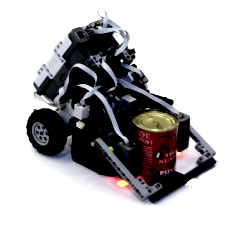
\includegraphics[width=7 cm]{zdjecia/FRANKIE.png}
	\caption{Robot Frankie \cite{ISTRO}}
	\label{fig:FRANKIE}
	\end{figure}

W stosunku do pozosta�ych robot�w jest on kompaktow� konstrukcj�. Nap�d zapewniaj� dwa zamocowane z ty�u serwomechanizmy. Rozwi�zaniem zastosowanym do unieruchamiania puszki podczas obrot�w jest ramka, nap�dzana przez serwomechanizm.

Jednostk� steruj�c� jest NXT Intelligent Brick. Poza 3 serwomechanizmami zastosowano tak�e czujnik odleg�o�ci (sprawdzaj�cy, czy puszka znajduje si� w odpowiednim miejscu) oraz 2 czujniki �wiat�a (odpowiadaj�ce za pod��anie za lini�). Robota zaopatrzono tak�e w dodatkowy, zewn�trzny akumulator.

Jego algorytm jazdy opiera si� na tym, �e puszki przez s�dzi�w dostawiane s� w te same miejsca. Po znalezieniu pierwszej puszki w pami�ci programu zapami�tywana jest jej pozycja, a nast�pnie robot ca�y czas zmierza w to samo miejsce. Pozwala to zminimalizowa� czas potrzebny na poszukiwanie puszki.
 
Co wi�cej, algorytm zastosowany w tym robocie jest dosy� niezawodny. Bardzo rzadko dochodzi�o do z�ego zinterpretowania sygna��w z czujnik�w. Umiejscowienie nap�d�w z ty�u, umo�liwi�o lepsze �ledzenie linii. Te wszystkie czynniki sprawi�y, �e ta konstrukcja bardzo dobrze radzi�a sobie w konkurencji z innymi robotami.

Nie ustrzeg�a si� jednak paru istotnych wad - nie jest wyposa�ona w �aden system pozycjonowania (np. magnetometr, akcelerometr itp.) przez co zupe�nie nie radzi sobie w sytuacjach nietypowych - np. podczas zderze�. 

\subsection{ARM Tank}

Robot ARM Tank zosta� skonstruowany przez Martin Povi�era (Czeskie Budziejowice, Czechy). Podobnie jak poprzednie konstrukcje, mo�na go sklasyfikowa� jako robota mobilnego klasy (2,0).
	\begin{figure}[H]
	\centering
	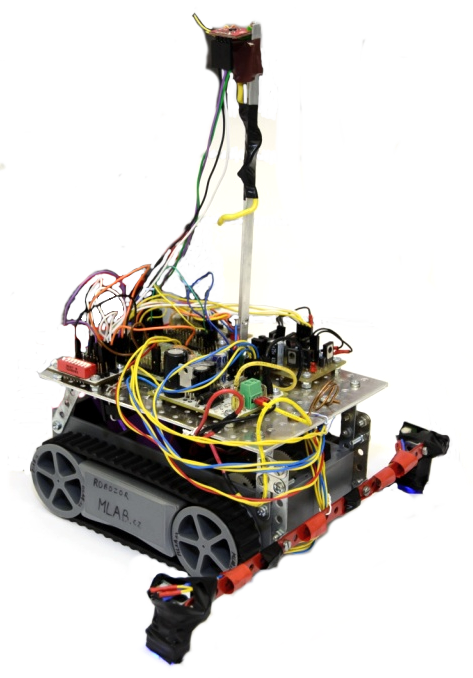
\includegraphics[width=9 cm]{zdjecia/ARMTANK.png}
	\caption{Robot ARM TANK \cite{ISTRO}}
	\label{fig:ARMTANK}
	\end{figure}
	
Jest to du�a i masywna konstrukcja. Spo�r�d innych robot�w w tej kategorii wyr�nia go zastosowanie nap�du g�siennicowego zamiast typowego nap�du ko�owego. Zastosowano w nich silniki DC z przek�adni� micro Pololu. Innym wyr�nikiem jest unikatowe podej�cie do kwestii unieruchamiania puszki - zdecydowano si� na zamocowanie 3 elektromagnes�w. 

Jednostk� steruj�c� robotem jest mikrokontroler STM32F107. Robot jest wyposa�ony w 9 transoptor�w odbiciowych: 7 w rozmieszczonych w linii, z przodu robota, odpowiadaj�cych za �ledzenie linii oraz 2 dodatkowe wspomagaj�ce cofanie. Z przodu robota zamocowano ultrad�wi�kowy czujnik odleg�o�ci. Dodatkowym czujnikiem jest umieszczony na swoistym wysi�gniku magnetometr, maj�cy za zadanie pom�c w okre�laniu orientacji robota. 

Robot najpierw lokalizuje miejsce w kt�rym znajduj� si� dostawiane przez organizator�w puszki. Po zebraniu  puszki robot cofa si� o jedno skrzy�owanie, a nast�pnie podje�d�a ponownie w to samo miejsce i przyci�ga kolejn� wolnym elektromagnesem. Po zebraniu 3 puszek robot cofa si� do linii bazowej i si� wy��cza.
 
Pomimo zastosowania wielu niesztampowych rozwi�za�, robot bardzo s�abo radzi� sobie podczas zawod�w. Najwi�kszym problemem by�o wy��czanie si� robota po zebraniu 3 puszek - inne konstrukcje wtedy mia�y wolne pole do popisu - nic nie przeszkadza�o im w swobodnym zebraniu pozosta�ych 11 puszek. Ponadto czasami da�o si� zaobserwowa� b��dy podczas zakr�t�w, prawdopodobnie zwi�zane z  problemami z magnetometrem - robot zawraca�, zamiast skr�ca�. Ponadto, elektromagnesy w jednym przypadku spowodowa�y zakleszczenie si� z innym robotem.


\subsection{Pomidor}

Robot Pomidor zosta� skonstruowany przez cz�onk�w Ko�a Naukowego Robotyk�w przy Wydziale MEiL Politechniki Warszawskiej. By�a to pierwsza tego typu konstrukcja, zbudowana jako platforma testowa oraz wyj�cie do p�niejszych modyfikacji. Mo�na go sklasyfikowa� jako robota mobilnego klasy (2, 0).

	\begin{figure}[H]
	\centering
	\includegraphics[width=11 cm]{zdjecia/POMIDOR.png}
	\caption{Robot Pomidor}
	\label{fig:POMIDOR}
	\end{figure}

Jest to dosy� du�a, cho� lekka i szybka konstrukcja. Opiera si� na dw�ch p�ytach laminatu szklano-epoksydowego, kt�ry pe�ni dwojak� rol� - po pierwsze stanowi podstaw� robota, po drugie s� na niej wytrawione po��czenia elektryczne. P�yty te s� ze sob� po��czone elementami dystansuj�cymi. W przedniej cz�ci robota znajduje si� wyci�cie mog�ce pomie�ci� trzy puszki. Ich wypadni�ciu poza obrys robota zapobiega ramka, nap�dzana przez serwomechanizm Dynamixel AX-12A. Nap�d robota zapewniaj� dwa silniki Pololu z mikro przek�adni� 30:1, zamocowane do dolnej podstawy robota. 

Jednostk� steruj�c� robotem jest mikrokontroler STM32F100RB, umieszczony w zestawie ewaluacyjnym STM32VL. Za poprawne wykrywanie linii odpowiada 7 transoptor�w odbiciowych KTIR0711S. Za wykrywanie puszek oraz przeciwnik�w odpowiadaj� 3 analogowe dalmierze SHARP GP2Y0A41SK0F. Aby zapewni� mo�liwo�� orientacji na planszy zastosowano w nim enkodery inkrementalne, dzia�aj�ce z wykorzystaniem transoptorach odbciowych. Robota wyposa�ono tak�e w modu� Bluetooth pozwalaj�cy na komunikacj� z komputerem (w celu debugowania b�d� monitorowania post�p�w).

Algorytm robota steruje robotem tak, aby odwiedza� on kolejno skrzy�owania D3 D5 C5 C1 B1 B5 A5 A1 D1 D3 (i tak dalej). W chwili znalezienia puszki (odczytania odpowiednio wysokiego wskazania na dalmierzach SHARP) robot zamyka ramk� tak, aby uniemo�liwi� utrat� kontaktu z puszk� np. przy zakr�tach lub przy cofaniu. Nast�pnie, znajduje skrzy�owanie na swojej linii bazowej, na kt�rym nie ma puszki (lub na kt�rym najdawniej odstawi� puszk�) i odwozi puszk� na to skrzy�owanie. Po zako�czeniu tej procedury, algorytm kontynuuje odwiedzanie kolejnych skrzy�owa�. Taki cykl powtarza si�, a� do zako�czenia rundy. 

Pomimo zastosowania du�ej ilo�ci czujnik�w, bardzo du�ej szybko�ci dzia�ania oraz interesuj�cego algorytmu, robot zaj�� na zawodach ISTROBOT dopiero czwarte miejsce. Dzia�o si� tak z powodu nieskutecznego rozpoznawania robota przeciwnika oraz niedostosowania konstrukcji do mo�liwo�ci zderzenia si� z innymi robotami.
	 

\chapter{Wnioski}

Celami pracy by�y:

\begin{itemize}
	\item zapoznanie si� z literatur� w zakresie robotyki mobilnej,
	\item wykonanie przegl�du rozwi�za� w zakresie budowy robot�w kategorii Ketchup House,
	\item okre�lenie wymaga� stawianych robotom Pomidor 1,5 oraz PACMAN,
	\item zaprojektowanie oraz wykonanie cz�ci mechanicznych robot�w Pomidor 1,5 oraz PACMAN,
	\item wykonanie �rodowiska testowego dla test�w czujnik�w oraz planszy zgodnej z regulaminami zawod�w, 
	\item przeprowadzenie test�w robot�w.
\end{itemize}

Wszystkie wyznaczone cele zosta�y zrealizowane.

W wyniku przeprowadzonych prac konstrukcyjnych powsta�y dwa roboty kategorii Ketchup House, spe�niaj�ce postawione za�o�enia konstrukcyjne. Roboty "POMIODR 1,5� oraz PACMAN zosta�y wyposa�one w szereg sensor�w umo�liwiaj�cych realizacj� algorytmu poruszania si� i zbierania puszek. 

Robot POMIDOR 1,5 zosta� W robocie POMIDOR 1,5 wyeliminowano wi�kszo�� b��d�w konstrukcyjnych wyst�puj�cych w robocie POMIDOR.


Robot PACMAN natomiast realizacj� koncepcji robota modu�owego - w kt�rym mo�na g��boko ingerowa� w jego budow�. Ponadto umo�liwia du�o szersze spektrum zastosowa�, np. jako robot inspekcyjny (przy wykorzystaniu modu�u wizyjnego), mapuj�cy pomieszczenie (z wykorzystaniem skanera 2D) b�d� interaktywno-pokazowy (przy zastosowaniu manipulatora). Jest to konstrukcja typowo prototypowa, niekt�re obszary funkcjonalno�ci wymagaj� dopracowania, jednak mo�na go potraktowa� jako przyczynek do rozwa�a� na temat tworzenia wielozadaniowych robot�w mobilnych. Prac� nad robotem zako�czono na etapie zaprojektowania cz�ci mechanicznej i elektronicznej. Dalszym krokiem w ramach pracy autora b�dzie  zintegrowanie robota z oprogramowaniem przygotowanym przez kol. Jakuba Pierewoja\cite{inzynierkaKuby} i przetestowanie jego dzia�a� na planszy w warunkach zbli�onych do zawod�w.

Dzi�ki wykonaniu pracy, autor zdoby� wiele nowych umiej�tno�ci:
\begin{itemize}
	\item zarz�dzanie ryzykiem,
	\item integrowanie cz�ci mechanicznej i elektronicznej,	
	\item projektowanie uk�ad�w mechanicznych i ich symulacja w �rodowisku Autodesk Inventor,
	\item projektowanie uk�ad�w elektronicznych w programie Altium Designer,
	\item wykonywanie element�w z wykorzystaniem drukarki 3D,,
	\item przeprowadzenie test�w robot�w.
\end{itemize}



\listoffigures
\listoftables

\begin{thebibliography}{1}
\bibitem{test1} Jezierski E., {\em Dynamika robot�w}, Wydawnictwa Naukowo-Techniczne, Warszawa 2006, str. 233-237
\bibitem{mataric}  Matari� M. J. {\em The Robotics Primer}, MIT Press, 2007
\bibitem{inzynierkaKuby} Pierewoj Jakub {\em Projekt i wykonanie robota mobilnego - oprogramowanie steruj�ce} 2015.
\bibitem{inzynierkaKaminskiego} Kami�ski Mateusz {\em Miniaturowy robot mobilny: projekt konstrukcji, wykonanie prototypu i oprogramowania} 2014.
\bibitem{LF} Ko�o Nauowe In�ynierii Mechatronicznej, \url{http://www.knim.pwr.wroc.pl/},  data dost�pu 20.01.2015
\bibitem{PUCK}  R-BOT, \url{http://r-bot.pl/index.php/zdjecia/} , data dost�pu 20.01.2015
\bibitem{ISTRO}  Istrobot, \url{http://www.robotika.sk/contest/2014/}, data dost�pu 20.01.2015
\bibitem{ROBOTIC}  Robotic Day, Ketchup House rules, \url{http://www.roboticday.org/}, data dost�pu 20.01.2015
\bibitem{KECZUP1} ISTROBOT, Ketchup House rules, \url{http://www.robotika.sk/contest/2014/EN/index.php?page=rules&type=ketchup}
\bibitem{KECZUP2} Regulamin zawod�w Robotic Day, \url{http://www.roboticday.org/2014/rules/2014-Ketchup_House-ENv1.pdf}, data dost�pu 20.01.2015
\bibitem{ROBOMATICON} Robomaticon, \url{http://robomaticon.pl/pl/node/45}, data dost�pu 20.01.2015
\bibitem{ROBOCHALLENGE} Robot Challenge, \url{http://www.robotchallenge.org/competition/}, data dost�pu 20.01.2015
\bibitem{POLOLU2212} Pololu, Product 2212  \url{http://www.pololu.com/product/2212}, data dost�pu 20.01.2015
\bibitem{POLOLU1090} Pololu, Product 1090  \url{http://www.pololu.com/product/1090}, data dost�pu 20.01.2015
\bibitem{POLOLU950} Pololu, Product 950	 \url{http://www.pololu.com/product/950}, data dost�pu 20.01.2015
\bibitem{POLOLU713} Pololu, Product 713  \url{http://www.pololu.com/product/713}, data dost�pu 20.01.2015
\bibitem{DYNAMIXEL} Dynamixel AX-12A, User�s Manual \url{http://www.electronickits.com/robot/BioloidAX-12(english).pdf}, data dost�pu 20.01.2015
\bibitem{STM32VL} STMicroelectronics, STM32 Discovery VL User's Manual \url{http://www.st.com/st-web-ui/static/active/jp/resource/technical/document/user_manual/CD00267113.pdf}, data dost�pu 20.01.2015
\bibitem{STM32F1}STMicroelectronics, STM32F100RB datasheet  \url{http://www.st.com/web/en/resource/technical/document/datasheet/CD00251732.pdf}, data dost�pu 20.01.2015
\bibitem{DUALSKY74} Botland, Dualsky 7,4 V \url{http://botland.com.pl/lipo-dualsky/2395-pakiet-lipol-dualsky-2200mah-25c-2s-74v-eco-s.html}, data dost�pu 20.01.2015
\bibitem{Sonar} Botland, HC-SR04 datasheet \url{http://botland.com.pl/index.php?controller=attachment&id_attachment=476}, data dost�pu 20.01.2015
\bibitem{SEN} Sparkfun, SEN-10530 datasheet \url{http://dlnmh9ip6v2uc.cloudfront.net/datasheets/Sensors/Magneto/HMC5883L-FDS.pdf}, data dost�pu 20.01.2015
\bibitem{LM339} Texas Instrument, LM339 datasheet \url{http://www.ti.com/lit/ds/symlink/lm339-n.pdf}, data dost�pu 20.01.2015
\bibitem{GP20} SHARP GP2Y0A41SK0 datasheet, \url{http://www.ti.com/lit/ds/symlink/lm339-n.pdf}, data dost�pu 20.01.2015
\bibitem{GP} SHARP GP2Y0D805Z0F  datasheet, \url{http://sharp-world.com/products/device/lineup/data/pdf/datasheet/gp2y0d805z_e.pdf}, data dost�pu 20.01.2015
\bibitem{KTIR} Kingbright, \url{http://www.kingbright.com/attachments/file/psearch/000/00/00/KTIR0711S(Ver.13).pdf}, data dost�pu 20.01.2015
\bibitem{POLOLU1442} Pololu, Product 1442 \url{http://www.pololu.com/product/1442}, data dost�pu 20.01.2015
\bibitem{DUALSKY11} Botland, Dualsky 11,1 V \url{http://botland.com.pl/lipo-dualsky/2487-pakiet-lipol-dualsky-3300mah-25c-2s-111v.html}, data dost�pu 20.01.2015
\bibitem{PRZETWORNICA} Pololu, Product 2110 \url{https://www.pololu.com/product/2110}, data dost�pu 20.01.2015
\bibitem{IRF} IRF4905 datasheet \url{http://www.redrok.com/MOSFET_IRF4905_-55V_-74A_20mO_Vth-4.0_TO-220.pdf}, data dost�pu 20.01.2015
\bibitem{VNH} ST Microelectronics, VNH5019ATR-E \url{http://www.st.com/st-web-ui/static/active/en/resource/technical/document/datasheet/CD00234623.pdf}, data dost�pu 20.01.2015
\bibitem{CNY} VISHAY, CNY70 datasheet \url{http://www.vishay.com/docs/83751/cny70.pdf}, data dost�pu 20.01.2015
\bibitem{HALL} Infineon Technologies AG, TLE4946-2K \url{http://www.infineon.com/dgdl/Infineon-TLE4946_2K-DS-v01_00-en.pdf?folderId=db3a30431f848401011facc1c83b4674&fileId=db3a30431f848401011fbc925c48637f}, data dost�pu 20.01.2015
\bibitem{PI} Raspberry Pi \url{http://www.raspberrypi.org/documentation/hardware/raspberrypi/}, data dost�pu 20.01.2015
\bibitem{PICAM} Raspberry PI HD Camera \url{http://www.raspberrypi.org/camera-board-available-for-sale/}, data dost�pu 20.01.2015
\bibitem{KLAW} TME, ACCORD KB1604-PAB \url{http://www.tme.eu/pl/details/kb1604-pab/klawiatury/accord/}, data dost�pu 20.01.2015
\bibitem{WYSW} Botland, wy�wietlacz 4x20 \url{http://botland.com.pl/wyswietlacze-alfanumeryczne/2640-wyswietlacz-lcd-4x20-znakow-niebieski-konwerter-i2c-lcm1602.html}, data dost�pu 20.01.2015
\bibitem{IMU} Pololu, Product 1264 \url{https://www.pololu.com/product/1264}, data dost�pu 20.01.2015
\bibitem{SKAN} Hokuyo, URG-04LX-UG01 \url{https://www.hokuyo-aut.jp/02sensor/07scanner/urg_04lx_ug01.html}, data dost�pu 20.01.2015
\bibitem{DAGU} DAGU Hi-Tech Electronic \url{http://dagurobot.diytrade.com/sdp/895152/4/pd-4555778/5252103-1798792/ROBOT_KIT_RA-001_SIX_SERVO_ROBOT_ARM.html}, data dost�pu 20.01.2015
\end{thebibliography} 

\end{document}
